\documentclass{article}

\usepackage{blindtext}
\usepackage[flushleft]{threeparttable}
\usepackage{booktabs}

\usepackage[capposition=top]{floatrow}


\usepackage{graphicx}

% bibliography
\usepackage[
backend=bibtex,
style=bwl-FU,
url=false,
doi=false,
eprint=false
]{biblatex}
\addbibresource{library.bib}


\begin{document}


\vspace*{3cm}

\begin{center}

\thispagestyle{empty}

{\Huge My first article}\\[0.5cm]
{\LARGE This is our first article using Latex}\\[1.5cm]

{\Large \bf Digital Tools for Finance}\\[1cm]

{\bf \large Fall Semester 2021\\
University of Zurich}\\[1cm]

{\large \bf \today }\\[3cm]


\begin{tabular}{ll}
\hline
{Authors (Student-ID):} & { Yaejin Kim (19-771-492)}\\
& { Philipp Pag (15-056-328)}\\
& { Matthias Hafner (08-055-741) }\\
\hline \\
\end{tabular}



\end{center}


\newpage


\section*{Abstract}
 
The purpose of this report is to examine the risk and return relation in the Swiss stock market. To reflect the Swiss stock market, the Swiss market index (SMI) has been chosen as the index of reference. This report is divided into three parts: Risk and Return, Portfolio Construction and Variance Ratios.

\newpage


\tableofcontents
\newpage

\section{Introduction}
\blindtext
\newpage

\section{Literatur Review}

\cite{Milgrom1982} and \cite{Gormsen2020} argue \blindtext
\newpage

\section{Results}


\begin{table} [!h] \centering 
	\begin{threeparttable}
		\caption{Value Portfolio}
     	\begin{tabular}{ccc}
        	\toprule
				    	& 01.01.1998 & 01.01.2008\\ 
			\midrule
			Nestle  	& Growth 	& Growth \\
			Roche 		& Growth 	& Growth \\ 
			UBS 		& Value 	& Growth \\
			Novartis 	& Growth 	& Growth \\ 
			\bottomrule
		\end{tabular}
		\footnotesize Note: Data collected using Bloomberg terminal.
	\end{threeparttable}
\end{table}

\blindtext

\begin{figure} [!h]
	\caption{Procedure of each treatment}
 	\begin{centering}
		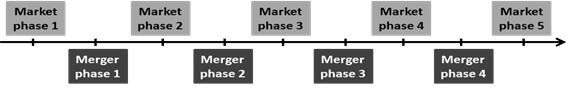
\includegraphics[width=0.8\linewidth]{phases} \\
	\end{centering}
	\footnotesize Note: Merger to monopoly not possible. In addtion, only one merger phase allowed. 
\end{figure}

\newpage

\section{Discussion}
\blindtext
\newpage







\section{References}
\begingroup
\renewcommand{\section}[2]{}
\nocite{*}
\printbibliography
\endgroup

\newpage




\end{document}
